\documentclass[12pt]{article}
\usepackage[hmargin=0.8in,vmargin=0.8in]{geometry}\usepackage[T1]{fontenc}
\usepackage{graphicx}\graphicspath{{images/}}
\usepackage{url}
\usepackage{indentfirst}

\setlength{\topskip}{0mm}\setlength{\parskip}{1em}\setlength{\parindent}{2em}
\usepackage{enumitem}\setlist{nolistsep}

\usepackage{natbib}
\setlength{\bibsep}{0.0pt}

\title{Pascal : A Natural Language Terminal}
\author{
  \IEEEauthorblockN{Eric Adamski}\\
  \IEEEauthorblockA{
    {\small School of Computer Science}\\
    {\small Carleton University}\\
    {\small Ottawa, Ontario, Canada}\\
    {\small Email: \{eric.adamski@cmail.carleton.ca\}}
  }
}
\date{\today}

\begin{document}
\maketitle

\begin{abstract}
  This report will discuss a natural language terminal in detail, what techniques were used, what language it is written in, and what libraries were used to make it possible. Since the original design is not perfect there are many newer schemes and technologies that do a better job at parsing commands, as an example, these techniques will also be discussed in future work to be done on the terminal. The program itself uses a naive bayesian classifier to classify different command structures, some results on accuracy will also be included. This is the first draft of the natural language terminal, and it is only in its infancy as not all functionality was implemented. This report will cover the current functionality of the terminal and future objectives as well.
\end{abstract}

\section{Introduction}

Use of low level computer commands is necessary for a computers function and commonly used by people whose profession revolves around computer systems. These core system commands are what has built modern computer software, and are still useful today. These commands and the interface from which they are used is foreign for inexperienced lay people. Having to learn and memorize computer commands for simple actions, which on modern systems have a graphical wrapper added for ease of use, seems disadvantageous. By creating a platform from which lay people can utilize the these commands, users would have a more personal relationship with their respective machine resulting in enhanced user experience. This would allow lay people to access powerful computer operations using their natural language which is more comfortable and convenient. That is why the natural language terminal has come into existence, make a low level computer interface accesable.

\subsection{Motivation}

The terminal will provide a more natural environment for inexperienced users of personal computers to interact via a comfortable medium. One will be able to communicate complex operations using natural language to the system and have it respond with easy to understand and properly formed english sentences. It will attempt to provide a more personal relationship with the machine via learning of the users behaviours and speech preferences.\cite{ogden} A simple example would be creating a directory, or folder, in a system. Normally an experienced user would understand the options of the 'mkdir' command, within the proposed system one could ask the system, "Could you please create a folder called NewFolder.", and the system will understand and execute the proper set of commands to complete the task. In the example above instead of saying, "... create a folder called NewFolder." one could also say, " ... create a folder named NewFolder.", so that any adjective which means to name could be used in place of named, or called. This feature would improve the overall user experience of the system by allowing the user some leeway when it comes to explaining their needs.\cite{kelly}

The use of computer terminals is reserved for those whose career is focused on computers. The objective of this system would be to open the use of computer terminals and their capabilities to the general public while building a more personal relationship and easing the use of these systems. Using natural language processing this system will allow the computer to build a relationship with its users and increase efficiency as well as the appeal of using low level computer commands. The remainder of this report will cover the a short background of how humans interact with computers, and a background on natural language processing and interactive systems, the method used to develop the natural language terminal and the libraries used, some testing results and future work related to this project.

\section{Background}

%background of humans and computers
How humans and computers interact has long been a focus of study\cite{biermann} and it continues to be at the forefront of research in academia and in the market for technology. Since the release of smaller more personalized computers there has been a push by consumers to make computers more accessible to all demographics. As computers have become integrated into everyday life for all it seems only logical to make them continuously easier to use, and even easier to adopt to the newer products. It has long been discussed that natural language would be the perfect medium to interact with computers, since the user has very little learning to do.\cite{kelly}\cite{aggarwal}\cite{ogden} This philosophy has been adopted by many companies in the 21\up{st} century. Apple Incorporated revolutionised the use of smart phones with their introduction of Siri, an interactive system which uses natural to communicate with the user. Not long after Microsoft followed up with their release of Cortana. Both of these interactive systems are voice activated and are part of the rising demand for hands free, easy to use, interactive technology. There are obviously many limits to both of the mentioned systems, but as time goes on and our understanding of how humans interact with computers increases so too will the knowledge and usability of Siri and Cortana and other natural language interfaces of computers.\cite{thompson}
%background on NLP


The ever growing field of natural language interfaces would be nothing without the our knowledge of how to interpret natural languages and process them into computer readable material. The history of natural language processing, or {\it NLP}, dates back to a paper written by Alan Turing in the mid 1950s.\footnote{\url{http://en.wikipedia.org/wiki/Natural_language_processing#History}} This paper also included the famed {\it Turing Test} which was designed to determine if a system which is being interacted with via questions is a human or computer. Up until the 1980s natural language processing consisted of matching strings of words with patterns and rules, which tended to be very complex in nature. Since then the field has turned to more of a machine learning approach, by which language structure and syntax is learned and possible inferred by the machine.\cite{socher} The system discussed throughout the rest of this report has made use of many {\it NLP} technologies and methods in order to create a more natural interactive system.

\section{Method}
\label{method}

The natural language terminal is a simple idea with a fairly complicated implementation. To implement an interface that allows a vast number of word combinations to mean the same thing was interesting and challenging. This section will discuss the tools used to build the terminal, the libraries and fields of research which helped bring the whole project together.

\subsection{Tools}

Since the terminal is going to be designed as a text base interface, a language needed to be selected which allowed for this. Ruby, being a scripting language, satisfied the requirement as well as added a few nice features that made the implementation better. Its seamless integration into any currently existing terminal program was the key reason it was selected, it also provided a functional style of programming which allowed for a smoother transition from written english text into executable pieces of code.\cite{matuszek} Another part of the Ruby language is that it is supported across many different operating systems with minimal setup required. All of the latter mentioned features of the language led to the use of Ruby as the main language for the system to be written.

Being a natural language terminal there was a need to be able to break down the english input and parse it into computer understandable pieces. This seemed too large of a feat for a single person to write an entire natural language processor, instead the vast amount of research and knowledge at Stanford help. Stanford has an entire open source library dedicated to processing natural language. Stanford NLP, as its known, and its Ruby language counterpart {\it Treat} played an enormous role in the success of implementing the terminal.

The last main tool that was used, and one of the most important parts of the entire system, allowed the machine to make decisions about the input given. There were many different classifiers that could have been chosen in the end it was simpler to use a naive bayesian classifier as it was taught by Dr. Oommen in class. After doing some more research into the specific area of translating natural language into command structed code\cite{matuszek}, it became clear that one of the poorest choices in creating this terminal was the classifier, which will be discussed further in section~\ref{Results}.
%how I wrote it
%%  - talk about Stanford NLP library and parse trees
%%  - talking about nieve bayseian classifier used for deciding

\subsection{Design & Implementation}

The idea behind the design of the terminal was to make it simple, a minimalist non-complicated interface. It resembles exactly the look of a classical computer terminal (see figure~\ref{figure_one}). The user then simply types a written english sentence or phrase designating the action the computer should execute.

\begin{figure}
  \centering
    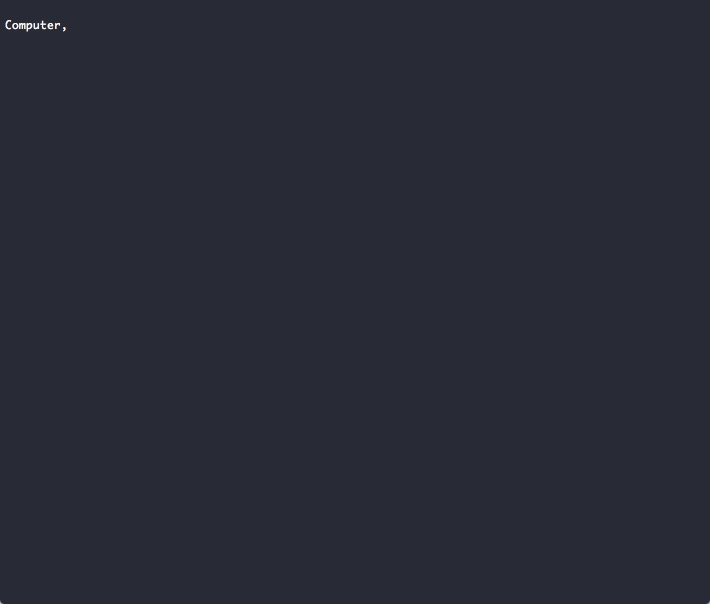
\includegraphics[width=\textwidth]{terminal}
  \caption{A snapshot of the interface of the natural language terminal.}
  \label{figure_one}
\end{figure}

After a phrase or command is entered the computer parses the sentence into a tree and decomposes the sentence into phrases, nouns, verbs, and so on. All stop words, {\it for the english language only}, are removed and the resulting words, referred to as \textbf{key words}, are sent to the computer {\it brain}. The {\it brain} of the terminal is where the classifier looks at the entire, non-parsed, phrase and classifies it into one of several categories of commands. One of the important parts of create the classifying system using a bayesian classifier was creating separate classes which can be differentiated by with only the use of {\it four} or {\it five} english words. The classifier, which is trained previously on a {\it corpus} of phrases, then has to classify the phrase as a {\it file, directory, display, command, or process} command. These classes where selected based on the component the resulting command will execute on. As an example, a {\it display} command would interact with the terminal user interface, as in the classical computer command {\it clear}. The terminal, as of now, supports {\it twenty one} basic terminal commands, most of which are original \textbf{UNIX} commands.

The class which have been chosen by the classifier then leads to the next layer of classification. Since the statements with the first level classifier are too similar, for example the statements "remove the directory ..." and "list the directory ..." only differ by a single word, and will be classified into the class {\it directory} as they both act on directory structure. The second tier classifier classifies within a class. In more of an english statement, once the brain chooses the phrase as a {\it file, directory, display, command, or process} command, it then chooses the exact command that needs to be executed. This two tier classification directed the implementation away from direct keyword matching.

After this process is complete, the brain takes the command which it has chosen as correct and executes it. Each command is stored in a structure which gives basic information about the command, the number of arguments that it takes, key words that it can match to (in the english language), the response which the computer will display to the user, and the exact command template which the program will use to execute the full command. This system of parsing and understanding english commands is very similar to a question answering system.\cite{aggarwal} The computer program needs to extract information about what the user is looking for with only minimal number of english words, about {\it three to five} english words after stopword removal. Since this is the case, and the fact that some commands are very similar in wording contribute to mistakes by the system.

\section{Results}
\label{Results}

After completing the implementation of the naive decision making portion of the natural language terminal some tests were run to determine the accuracy of classification by the system. {\it Eighty five} different phrases were given to the terminal one at a time. The corresponding command was compared to the one given by the {\it brain's} classification system. The results are not surprising, and actually are reasonable given the system for classifying. In table~\ref{table_results} a handful of the results are shown, the '\textbf{Classification Result}' column is the result back from the computer, the '\textbf{Proper Result}' column is the proper classification. A result of {\it No Classification} means the phrase could not be classified into one of the command classes. Overall the classification accuracy was {\it 67\%}. Since the classification was fairly low, some parts of the full functionality where left out at this stage.

\begin{table}
  \centering
    \begin{tabular}{ | l | c | r | }
      \hline
      Classification Result & Proper Result & Correct \\ \hline
      find & ls	& No \\ \hline
      clear	& clear	& Yes \\ \hline
      cd & cd	& Yes \\ \hline
      touch	& touch	& Yes \\ \hline
      find & find	& Yes \\ \hline
      find & find & Yes \\ \hline
      find & mv & No \\ \hline
      diff & diff & Yes \\ \hline
      find & find & Yes \\ \hline
      exec & exec	& Yes \\ \hline
      rmdir	& pwd & No \\ \hline
      No Classification	& clear & No \\ \hline
      No Classification	& whoami & No \\ \hline
      ln & ln & Yes \\ \hline
      cp & cp & Yes \\ \hline
      No Classification & pwd & No \\ \hline
      mkdir & mkdir & Yes \\ \hline
      cat & cat & Yes \\ \hline
      grep & grep & Yes \\ \hline
      cp & cp & Yes \\ \hline
      diff & diff & Yes \\ \hline
      rmdir & pwd & No \\ \hline
      cat & cat & Yes \\ \hline
      mkdir & mv & No \\ \hline
      ln & ln & Yes \\ \hline
      file & touch & No \\ \hline
      echo & echo & Yes \\ \hline
      exec & exec & Yes \\ \hline
      man & man & Yes \\ \hline
      man & man & Yes \\ \hline
      rmdir & rmdir & Yes \\ \hline
      file & touch & No \\ \hline
      exec & exec & Yes \\ \hline
      cat & cat & Yes \\ \hline
      find & find & Yes \\ \hline
      file & touch & No \\ \hline
    \end{tabular}
    \caption{A sample of classification results for a set of 85 tests, resulting in 67.06\% accuracy. }
    \label{table_results}
\end{table}

\section{Furture Work}

As mentioned in sections~\ref{Results} and \ref{method} there were features which were not included in this implementation of the terminal. The ability to parse arguments from english sentences is a large portion that was left out. This is due to the inconsistent location of valuable information in an english phrase of sentence. In any future work this feature is essential to make the terminal useful.

After completing the classification system in the {\it brain} some better systems to classify and parse command structures from english sentences into executable code was found in \cite{matuszek}. A Uniform Based Learner, or {\it UBL} in conjunction with a version of combinatory categorial grammars, or {\it CCGs}, which helps narrow and infer the structure of phrases would be implemented in any future work on this project. Due to the time limit this wasn't able to be accomplished but would be the main focus before any new features were to be included in the product.
% different techniques (taken from \cite{matuszek})

\section{Conclusion}

Overall the experience of building such a system was magnificent. Although the system is not complete, the phase which it is at allows for natural language sentences to control a simple computer terminal. Time permitting some redesign of the classification system to use a {\it UBL} and a {\it CCG} instead of the naive bayesian classifier. The question in the end would be, 'Has it made using a computer terminal easier and more accessible to those not comfortable with computers?' and at this point I think it actually makes no difference, as the syntax and structure of the computer and its original commands are no different when representing them in their original form. That being said, if a system were to be included which would make it more personable and helpful, instead of just a plain interface, to walk users through the process of executing a command and providing the necessary information, I think this system could open the use of these commands to less knowledgeable people.

All the code and the '.tex' files for this document are open source available here\footnote{\url{https://github.com/ericadamski/nlTerminal}}, you will also find the instructions on how to start and stop the terminal on the link. Note that because of the {\it 67\%} accuracy of the system, the commands never get executed so not to mess up or remove files or directories on the machine.

\bibliographystyle{abbrv}
\bibliography{references}

\end{document}
